

\tikzset{every picture/.style={line width=0.75pt}} %set default line width to 0.75pt        

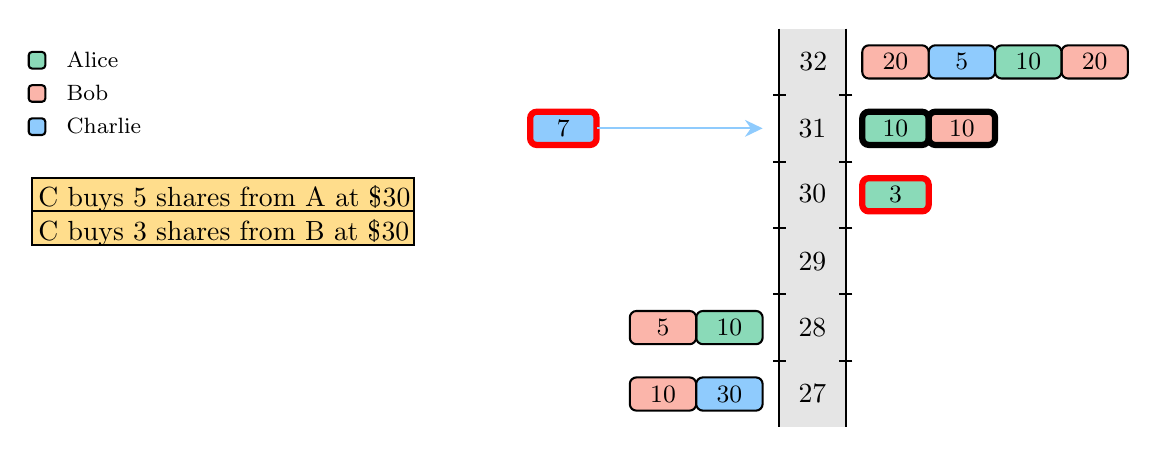
\begin{tikzpicture}[x=0.75pt,y=0.75pt,yscale=-0.8,xscale=0.8]
%uncomment if require: \path (0,300); %set diagram left start at 0, and has height of 300


%Shape: Rectangle [id:dp0819038861204413] 
\draw  [draw opacity=0][fill={rgb, 255:red, 0; green, 0; blue, 0 }  ,fill opacity=0.1 ] (480,30) -- (520,30) -- (520,270) -- (480,270) -- cycle ;
%Straight Lines [id:da11910476519653257] 
\draw    (480,30) -- (480,270) (484,70) -- (476,70)(484,110) -- (476,110)(484,150) -- (476,150)(484,190) -- (476,190)(484,230) -- (476,230) ;
%Straight Lines [id:da6345525229446171] 
\draw    (520,30) -- (520,270) (524,70) -- (516,70)(524,110) -- (516,110)(524,150) -- (516,150)(524,190) -- (516,190)(524,230) -- (516,230) ;
%Rounded Rect [id:dp5841732804090376] 
\draw  [color={rgb, 255:red, 255; green, 0; blue, 0 }  ,draw opacity=1 ][fill={rgb, 255:red, 138; green, 218; blue, 184 }  ,fill opacity=1 ][line width=2.25]  (530,124) .. controls (530,121.79) and (531.79,120) .. (534,120) -- (566,120) .. controls (568.21,120) and (570,121.79) .. (570,124) -- (570,136) .. controls (570,138.21) and (568.21,140) .. (566,140) -- (534,140) .. controls (531.79,140) and (530,138.21) .. (530,136) -- cycle ;
%Rounded Rect [id:dp1834680548544293] 
\draw  [color={rgb, 255:red, 0; green, 0; blue, 0 }  ,draw opacity=1 ][fill={rgb, 255:red, 138; green, 218; blue, 184 }  ,fill opacity=1 ][line width=2.25]  (530,84) .. controls (530,81.79) and (531.79,80) .. (534,80) -- (566,80) .. controls (568.21,80) and (570,81.79) .. (570,84) -- (570,96) .. controls (570,98.21) and (568.21,100) .. (566,100) -- (534,100) .. controls (531.79,100) and (530,98.21) .. (530,96) -- cycle ;
%Rounded Rect [id:dp9540702911156453] 
\draw  [fill={rgb, 255:red, 138; green, 218; blue, 184 }  ,fill opacity=1 ][line width=0.75]  (430,204) .. controls (430,201.79) and (431.79,200) .. (434,200) -- (466,200) .. controls (468.21,200) and (470,201.79) .. (470,204) -- (470,216) .. controls (470,218.21) and (468.21,220) .. (466,220) -- (434,220) .. controls (431.79,220) and (430,218.21) .. (430,216) -- cycle ;
%Rounded Rect [id:dp11917240068278401] 
\draw  [fill={rgb, 255:red, 251; green, 181; blue, 170 }  ,fill opacity=1 ][line width=0.75]  (390,204) .. controls (390,201.79) and (391.79,200) .. (394,200) -- (426,200) .. controls (428.21,200) and (430,201.79) .. (430,204) -- (430,216) .. controls (430,218.21) and (428.21,220) .. (426,220) -- (394,220) .. controls (391.79,220) and (390,218.21) .. (390,216) -- cycle ;
%Rounded Rect [id:dp7245467196534818] 
\draw  [fill={rgb, 255:red, 251; green, 181; blue, 170 }  ,fill opacity=1 ][line width=0.75]  (390,244) .. controls (390,241.79) and (391.79,240) .. (394,240) -- (426,240) .. controls (428.21,240) and (430,241.79) .. (430,244) -- (430,256) .. controls (430,258.21) and (428.21,260) .. (426,260) -- (394,260) .. controls (391.79,260) and (390,258.21) .. (390,256) -- cycle ;
%Rounded Rect [id:dp03827927607995818] 
\draw  [fill={rgb, 255:red, 138; green, 218; blue, 184 }  ,fill opacity=1 ][line width=0.75]  (28,46) .. controls (28,44.9) and (28.9,44) .. (30,44) -- (36,44) .. controls (37.1,44) and (38,44.9) .. (38,46) -- (38,52) .. controls (38,53.1) and (37.1,54) .. (36,54) -- (30,54) .. controls (28.9,54) and (28,53.1) .. (28,52) -- cycle ;
%Rounded Rect [id:dp7222729266059345] 
\draw  [fill={rgb, 255:red, 143; green, 203; blue, 253 }  ,fill opacity=1 ][line width=0.75]  (28,86) .. controls (28,84.9) and (28.9,84) .. (30,84) -- (36,84) .. controls (37.1,84) and (38,84.9) .. (38,86) -- (38,92) .. controls (38,93.1) and (37.1,94) .. (36,94) -- (30,94) .. controls (28.9,94) and (28,93.1) .. (28,92) -- cycle ;
%Rounded Rect [id:dp3636132794332668] 
\draw  [fill={rgb, 255:red, 251; green, 181; blue, 170 }  ,fill opacity=1 ][line width=0.75]  (28,66) .. controls (28,64.9) and (28.9,64) .. (30,64) -- (36,64) .. controls (37.1,64) and (38,64.9) .. (38,66) -- (38,72) .. controls (38,73.1) and (37.1,74) .. (36,74) -- (30,74) .. controls (28.9,74) and (28,73.1) .. (28,72) -- cycle ;
%Rounded Rect [id:dp46209137558796687] 
\draw  [color={rgb, 255:red, 0; green, 0; blue, 0 }  ,draw opacity=1 ][fill={rgb, 255:red, 251; green, 181; blue, 170 }  ,fill opacity=1 ][line width=2.25]  (570,84) .. controls (570,81.79) and (571.79,80) .. (574,80) -- (606,80) .. controls (608.21,80) and (610,81.79) .. (610,84) -- (610,96) .. controls (610,98.21) and (608.21,100) .. (606,100) -- (574,100) .. controls (571.79,100) and (570,98.21) .. (570,96) -- cycle ;
%Rounded Rect [id:dp866142470002609] 
\draw  [fill={rgb, 255:red, 143; green, 203; blue, 253 }  ,fill opacity=1 ][line width=0.75]  (570,44) .. controls (570,41.79) and (571.79,40) .. (574,40) -- (606,40) .. controls (608.21,40) and (610,41.79) .. (610,44) -- (610,56) .. controls (610,58.21) and (608.21,60) .. (606,60) -- (574,60) .. controls (571.79,60) and (570,58.21) .. (570,56) -- cycle ;
%Rounded Rect [id:dp708981159795911] 
\draw  [fill={rgb, 255:red, 143; green, 203; blue, 253 }  ,fill opacity=1 ][line width=0.75]  (430,244) .. controls (430,241.79) and (431.79,240) .. (434,240) -- (466,240) .. controls (468.21,240) and (470,241.79) .. (470,244) -- (470,256) .. controls (470,258.21) and (468.21,260) .. (466,260) -- (434,260) .. controls (431.79,260) and (430,258.21) .. (430,256) -- cycle ;
%Rounded Rect [id:dp7591462434368331] 
\draw  [color={rgb, 255:red, 255; green, 0; blue, 0 }  ,draw opacity=1 ][fill={rgb, 255:red, 143; green, 203; blue, 253 }  ,fill opacity=1 ][line width=2.25]  (330,84) .. controls (330,81.79) and (331.79,80) .. (334,80) -- (366,80) .. controls (368.21,80) and (370,81.79) .. (370,84) -- (370,96) .. controls (370,98.21) and (368.21,100) .. (366,100) -- (334,100) .. controls (331.79,100) and (330,98.21) .. (330,96) -- cycle ;
%Straight Lines [id:da013136060541545924] 
\draw [color={rgb, 255:red, 143; green, 203; blue, 253 }  ,draw opacity=1 ]   (370,90) -- (467,90) ;
\draw [shift={(470,90)}, rotate = 180] [fill={rgb, 255:red, 143; green, 203; blue, 253 }  ,fill opacity=1 ][line width=0.08]  [draw opacity=0] (10.72,-5.15) -- (0,0) -- (10.72,5.15) -- (7.12,0) -- cycle    ;
%Rounded Rect [id:dp0037524200066810787] 
\draw  [fill={rgb, 255:red, 251; green, 181; blue, 170 }  ,fill opacity=1 ][line width=0.75]  (530,44) .. controls (530,41.79) and (531.79,40) .. (534,40) -- (566,40) .. controls (568.21,40) and (570,41.79) .. (570,44) -- (570,56) .. controls (570,58.21) and (568.21,60) .. (566,60) -- (534,60) .. controls (531.79,60) and (530,58.21) .. (530,56) -- cycle ;
%Rounded Rect [id:dp15509522152906374] 
\draw  [fill={rgb, 255:red, 251; green, 181; blue, 170 }  ,fill opacity=1 ][line width=0.75]  (650,44) .. controls (650,41.79) and (651.79,40) .. (654,40) -- (686,40) .. controls (688.21,40) and (690,41.79) .. (690,44) -- (690,56) .. controls (690,58.21) and (688.21,60) .. (686,60) -- (654,60) .. controls (651.79,60) and (650,58.21) .. (650,56) -- cycle ;
%Rounded Rect [id:dp31347310397506256] 
\draw  [fill={rgb, 255:red, 138; green, 218; blue, 184 }  ,fill opacity=1 ][line width=0.75]  (610,44) .. controls (610,41.79) and (611.79,40) .. (614,40) -- (646,40) .. controls (648.21,40) and (650,41.79) .. (650,44) -- (650,56) .. controls (650,58.21) and (648.21,60) .. (646,60) -- (614,60) .. controls (611.79,60) and (610,58.21) .. (610,56) -- cycle ;
%Shape: Rectangle [id:dp14290409086582512] 
\draw  [fill={rgb, 255:red, 255; green, 221; blue, 140 }  ,fill opacity=1 ] (30,120) -- (260,120) -- (260,140) -- (30,140) -- cycle ;
%Shape: Rectangle [id:dp6436928446902445] 
\draw  [fill={rgb, 255:red, 255; green, 221; blue, 140 }  ,fill opacity=1 ] (30,140) -- (260,140) -- (260,160) -- (30,160) -- cycle ;

% Text Node
\draw (500,90) node    {$31$};
% Text Node
\draw (500,129.5) node    {$30$};
% Text Node
\draw (500,170) node    {$29$};
% Text Node
\draw (500,210) node    {$28$};
% Text Node
\draw (500,250) node    {$27$};
% Text Node
\draw (550,130) node  [font=\small]  {$3$};
% Text Node
\draw (550,90) node  [font=\small]  {$10$};
% Text Node
\draw (450,210) node  [font=\small]  {$10$};
% Text Node
\draw (410,210) node  [font=\small]  {${\textstyle 5}$};
% Text Node
\draw (410,250) node  [font=\small]  {$10$};
% Text Node
\draw (49,42) node [anchor=north west][inner sep=0.75pt]  [font=\footnotesize] [align=left] {Alice};
% Text Node
\draw (49,62) node [anchor=north west][inner sep=0.75pt]  [font=\footnotesize] [align=left] {Bob};
% Text Node
\draw (49,82) node [anchor=north west][inner sep=0.75pt]  [font=\footnotesize] [align=left] {Charlie};
% Text Node
\draw (590,90) node  [font=\small]  {$10$};
% Text Node
\draw (500.5,50) node    {$32$};
% Text Node
\draw (590,50) node  [font=\small]  {$5$};
% Text Node
\draw (450,250) node  [font=\small]  {$30$};
% Text Node
\draw (350,90) node  [font=\small]  {$7$};
% Text Node
% Text Node
\draw (550,50) node  [font=\small]  {$20$};
% Text Node
\draw (670,50) node  [font=\small]  {$20$};
% Text Node
\draw (630,50) node  [font=\small]  {$10$};
% Text Node
\draw (32,123) node [anchor=north west][inner sep=0.75pt]   [align=left] {C buys 5 shares from A at \$30};
% Text Node
\draw (32,143) node [anchor=north west][inner sep=0.75pt]   [align=left] {C buys 3 shares from B at \$30};


\end{tikzpicture}
